%%%%%%%%%%%%%%%%%%%%%%%%%%%%
% Two Sword Lengths
% Christopher Gandrud
% 28 June 2013
%%%%%%%%%%%%%%%%%%%%%%%%%%%%

% !Rnw weave = knitr

\documentclass[a4paper]{article}\usepackage{graphicx, color}
%% maxwidth is the original width if it is less than linewidth
%% otherwise use linewidth (to make sure the graphics do not exceed the margin)
\makeatletter
\def\maxwidth{ %
  \ifdim\Gin@nat@width>\linewidth
    \linewidth
  \else
    \Gin@nat@width
  \fi
}
\makeatother

\definecolor{fgcolor}{rgb}{0.2, 0.2, 0.2}
\newcommand{\hlnumber}[1]{\textcolor[rgb]{0,0,0}{#1}}%
\newcommand{\hlfunctioncall}[1]{\textcolor[rgb]{0.501960784313725,0,0.329411764705882}{\textbf{#1}}}%
\newcommand{\hlstring}[1]{\textcolor[rgb]{0.6,0.6,1}{#1}}%
\newcommand{\hlkeyword}[1]{\textcolor[rgb]{0,0,0}{\textbf{#1}}}%
\newcommand{\hlargument}[1]{\textcolor[rgb]{0.690196078431373,0.250980392156863,0.0196078431372549}{#1}}%
\newcommand{\hlcomment}[1]{\textcolor[rgb]{0.180392156862745,0.6,0.341176470588235}{#1}}%
\newcommand{\hlroxygencomment}[1]{\textcolor[rgb]{0.43921568627451,0.47843137254902,0.701960784313725}{#1}}%
\newcommand{\hlformalargs}[1]{\textcolor[rgb]{0.690196078431373,0.250980392156863,0.0196078431372549}{#1}}%
\newcommand{\hleqformalargs}[1]{\textcolor[rgb]{0.690196078431373,0.250980392156863,0.0196078431372549}{#1}}%
\newcommand{\hlassignement}[1]{\textcolor[rgb]{0,0,0}{\textbf{#1}}}%
\newcommand{\hlpackage}[1]{\textcolor[rgb]{0.588235294117647,0.709803921568627,0.145098039215686}{#1}}%
\newcommand{\hlslot}[1]{\textit{#1}}%
\newcommand{\hlsymbol}[1]{\textcolor[rgb]{0,0,0}{#1}}%
\newcommand{\hlprompt}[1]{\textcolor[rgb]{0.2,0.2,0.2}{#1}}%

\usepackage{framed}
\makeatletter
\newenvironment{kframe}{%
 \def\at@end@of@kframe{}%
 \ifinner\ifhmode%
  \def\at@end@of@kframe{\end{minipage}}%
  \begin{minipage}{\columnwidth}%
 \fi\fi%
 \def\FrameCommand##1{\hskip\@totalleftmargin \hskip-\fboxsep
 \colorbox{shadecolor}{##1}\hskip-\fboxsep
     % There is no \\@totalrightmargin, so:
     \hskip-\linewidth \hskip-\@totalleftmargin \hskip\columnwidth}%
 \MakeFramed {\advance\hsize-\width
   \@totalleftmargin\z@ \linewidth\hsize
   \@setminipage}}%
 {\par\unskip\endMakeFramed%
 \at@end@of@kframe}
\makeatother

\definecolor{shadecolor}{rgb}{.97, .97, .97}
\definecolor{messagecolor}{rgb}{0, 0, 0}
\definecolor{warningcolor}{rgb}{1, 0, 1}
\definecolor{errorcolor}{rgb}{1, 0, 0}
\newenvironment{knitrout}{}{} % an empty environment to be redefined in TeX

\usepackage{alltt}
\usepackage{fullpage}
\usepackage{lscape}
\usepackage[authoryear]{natbib}
\usepackage{setspace}
    \doublespacing
\usepackage{hyperref}
\hypersetup{
    colorlinks,
    citecolor=black,
    filecolor=black,
    linkcolor=cyan,
    urlcolor=cyan
}
\usepackage{booktabs}
\usepackage{dcolumn}
\usepackage{url}
\usepackage{tikz}
\usepackage{todonotes}
\usepackage{verbatim}
\usepackage{endnotes}


\setlength{\belowcaptionskip}{0.5cm}

%%%%%%% Title Page %%%%%%%%%%%%%%%%%%%%%%%%%%%%%%%%%%%%%%%%%%%%
\title{Two Sword Lengths: Violence in Elected National Legislatures}

\author{Christopher Gandrud \\
                {\emph{Hertie School of Governance}}\endnote{Research Associate. Friedrichstra{\ss}er 180. 10117 Berlin, Germany. Email: \href{mailto:christopher.gandrud@gmail.com}{christopher.gandrud@gmail.com}. Thank you to Emily Beaulieu and Simon Hix for very helpful comments, Hortense Badarani for research assistance, seminar participants at Yonsei University, and my students at the LSE for inspiration.}}
\date{}
\IfFileExists{upquote.sty}{\usepackage{upquote}}{}

\begin{document}

\maketitle

%%%%%%% Abstract %%%%%%%%%%%%%%%%%%%%%%%%%%%%%%%%%%%%%%%%%%%%
\begin{abstract}
Elected national legislative chambers should be venues for peacefully resolving conflicts between opposing groups. However, they can sometimes become the scenes of physical violence between legislators. Legislative violence is an indication that a country's democratic institutions are functioning far from perfectly as legislative actors are deciding to drop out of the `game', rather than follow the rules. In this first global study of legislative violence, I argue that violence is more likely when legislators do not view the prevailing nonviolent rules as fair and are therefore illegitimate. Perceived fairness and legitimacy are higher in countries with highly proportional electoral outcomes and established democracies. I use a new global data set of legislative violence from the 1980s through Winter 2011 to test this assertion. I find robust evidence that legislative violence is more prevalent in countries with disproportionate electoral outcomes and in new democracies. Furthermore, the analysis suggests that having both a new democracy and all but very high proportionality may be necessary for legislative violence.
\end{abstract}


\paragraph{Keywords:} legislatures, violence, electoral proportionality, institutional design, majority and minority governments

\vspace{0.3cm}

%%%%%%% Introduction %%%%%%%%%%%%%%%%%%%%%%%%%%%%%%%%%%%%%%%%%%%%

Though legislators are often described as `battling' or `fighting' in democracies we generally expect these battles to be in terms of rhetoric and procedural maneuvers circumscribed by rules and norms that culminate in votes. The outcomes of these contests are then respected by all legislators. Unfortunately, metaphorical battles sometimes become physical fights between members of legislatures. 

The history of many legislative chambers contains incidents of violence between legislators. In 1856 a member of the United States House of Representatives, canned a senator unconscious in the Senate chamber in a dispute over slavery \citep{USSenateCanning}. It has been suggested that the United Kingdom's House of Commons is physically designed to prevent violence between members. The Government and Opposition benches are said to be ``two sword lengths apart" \citep{ParliamentUKSword} so that duels will be fought with words rather than swords. Actual, sword fights do not seem to have taken place in the Commons chamber, but violent incidences did occur. For example, in 1893 a fight broke out between Irish nationalist and Unionist members of parliament \citep{ByrneViolence}. Violence in legislatures continues to occur, with incidences being regularly reported on by the media.\endnote{The Guardian newspaper, for example, sporadically compiles stories of physical fights in legislative chambers. See \url{http://www.guardian.co.uk/politics/gallery/2010/dec/17/1\#/?picture=369861052\&index=0}. Legislative violence has also has its own Wikipedia page. See {\url{http://en.wikipedia.org/wiki/Legislative_violence}}.} Recent instances of violence between legislators include multiple brawls in Ukraine in 2010 and in South Korea in 2009. In both cases opposition legislators, facing impending legislative defeats, tried to obstruct the governments' attempts to pass controversial legislation.\endnote{In Ukraine the fight was over Russian military bases and in South Korea it concerned media ownership laws.} Even more recently in 2013 a large confrontation occurred in the Venezuelan National Assembly when the Assembly President withheld speaking time from legislators who did not recognized the victory of the new president in a very highly contested election.

Until recently legislative disruption, of which violence is an extreme example, has been largely ignored by political scientists.\endnote{A recent special issue of \emph{Democratization} \citeyearpar{Democratization2013} entitled \emph{Disruptive Democracy: Analysing Legislative Protest} has made a persuasive case that it deserves scholarly attention. Indeed, these acts reflect ``political conflict as well as systemic issues in democratic and democratizing institutional contexts'' \citep[394-395]{Spary2013}.} Though legislative disruption in general is not necessarily `good' or `bad' \citep[see][for discussions of how disruption may be a `safety valve' in contexts where dissent is strongly curtailed]{Ostrow1996,Young2002}, legislative violence does symbolize a dramatic break from scholars' assumption that compliance with legislative rules of the `game' is a given \cite{Wolfe2004}. Some single-country case study work has been done on--mostly nonviolent--legislative disruption \cite[see][]{Armitage2013,Johnson2013,Ilie2013,Wolfe2004} and other work has examined the strategic choices politicians make when they choose to not participate in the democratic rules of the game \citep[e.g.][on election boycotts]{Beaulieu2008}. In this paper I am interested in expanding this work to understand legislative violence in elected national assemblies on a global scale. Indeed, this paper includes the first global description of violence between legislators. 

In this paper I first develop a framework for understanding when legislative violence in elected legislatures is more likely. I propose that when members of parliament view legislative procedures to be unfair and therefore illegitimate the probability of violence is higher. I argue that at least two factors are very important for determining legislators' perceptions of fairness and legitimacy: the \emph{proportionality of a country's electoral outcomes} and the \emph{age of its democracy}. Legislators in countries with very proportional outcomes and older democracies will be more likely to view legislative rules as fair, legitimate, and therefore worth adhering to, at least to the extent that they don't use the most extreme form of legislative disruption--violence. 

In this paper, after developing my framework and a number of key alternative explanations, I describe violence in national legislatures around the world with a new data set of from 1980 through Winter 2011. In this section I also demonstrate simple association between my key framework variables and violence. I then undertake a further investigation by discussing the variables and rare event logistic regression models \citep{KingRareEvents2001, KingRareEventsPA2001} I use to study these (thankfully) rare events. Finally, I lay out my finding that there is robust evidence that legislative violence is more prevalent in countries with disproportionate electoral outcomes, in new democracies, and in countries with low societal-level trust. Furthermore, the analysis suggests that having both highly disproportionate electoral outcomes and a new democracy may be necessary for legislative violence.

%%%%%%%%%%%%%%%%%%%%%%%%%%%%%%%%%%%%%%%%%%%%%% Previous Research & Framework

\section{A Framework for Understanding Legislative Violence}

Contestation is a key function of legislatures and democracies \citep{Alvarez1996, Dahl1971, Follesdal2006} and creates winners and losers. Indeed democracy, ``is a system in which parties lose elections" \citep[][10]{Przeworski1991}. When contestation is nonviolent and rule bound, losers and winners consent to follow them \citep[c.f.][]{Anderson2005}. However, when violence between legislators in the parliamentary chamber occurs at least some legislators do not believe that voting and other parliamentary procedures, or at least the current implementation of the procedures is legitimate. They are not `playing by the rules of the game', but instead taking extreme extra-procedural actions to influence outcomes.

My main assertion is that violence is less likely when legislators view their parliament's procedures as fair. Perceived fairness has been shown to be an important component of people's perceptions of legitimacy across a wide range of settings \citep[see][]{thibaut1975,Tyler2001,Tyler2006}. The more fair people view procedures to be, the more likely they are to view them as legitimate and worth complying with even if they do not directly benefit from an outcome. So, the more fair and therefore legitimate legislators view their legislature to be, the more likely they are to comply with the nonviolent legislative rules and norms of the game. 

Under what conditions do legislators decide that the rules are not legitimate and choose to use violence rather than comply with them? I focus on two observable--at the global level, the level of this study--factors that could influence legislators' views of legislative rule legitimacy: proportionality of electoral outcomes and age of democracy. 

Note that this is far from a complete account of all of the factors that may influence perceptions of fairness and legitimacy. \cite{Wolfe2004} for example focuses on informal ways that opposition parties can access power, heightening a minority legislators' perceptions of fairness and willingness to comply with parliamentary procedures. Given the global scale of this paper proportionality of electoral outcomes and age of democracy are much more easily observable. Further complementary case study research is needed to understand other facets.

\paragraph{Proportional Electoral Outcomes}

Possibly the most important component of whether or not legislators view their legislature as fair and legitimate is the proportionality of the election that allocated its seats. Proportional electoral outcomes--where parties' proportion of seats won closely corresponds to their proportion of votes won--are widely regarded as more fair \citep{norris1997}. The difference in the ratios of winning parties' and losing parties' seats to votes shares\endnote{If the ratio equals one then the proportion of seats that a party wins is equal to its proportion of votes.} is much smaller when there are proportional rather than disproportional outcomes. Losers may be more likely to view legislative outcomes as illegitimate if they are created by winners whose representation is much larger than their vote shares \citep[see][]{lijphart1999}.\footnote{\cite{CHO2006} find that in Lesotho, while smaller party partisan voters were more satisfied with proportional outcomes, those who support larger `winning' parties tended to become less satisfied with a more proportional outcome. They argue that more proportional electoral system promote a convergence in satisfaction between winners and losers. The key here is that the point of convergence be above a threshold where parliamentarians would view legislative procedures as so unfair and illegitimate that they would use violence.} Consenting to these rules of the game established and administered by winners of an electorally disproportionately large legislative majority could be harder, so violence is more likely.

How proportional is proportional enough to promote widespread feelings of fairness among legislators to the extent that they refrain from using violence? \cite{Marien2011} found that there was a curvilinear relationship between proportional electoral outcomes and citizens' political trust. Feelings of political trust were highest for very proportional systems\endnote{The most trusting societies had Gallagher disproportionality scores of close to 1. See the discussion below for further details about this measure.} and very disproportional or majoritarian systems. Countries in the middle had the lowest trust.\endnote{Outcomes in the middle may be a ``bastard-producing hybrid'' \citep[74]{Sartori1994} that combines the defects of both highly proportional and disproportional outcomes.} Should we expect a similar curvilinear relationship for legislators' sense of fairness? Probably not. Marien argues that high trust at the low end of disproportionality is caused by the reasons we have discussed so far regarding fairness. Political trust is promoted by the fairness of electoral outcomes \citep{lijphart1999}. However, she argues that high voter trust in very disproportionate countries is caused by something different: high accountability. Disproportional majoritarian elections produce highly accountable legislatures where citizens feel a strong sense of control over their politicians \citep{Aarts2008,CHO2012}. Though this characteristic may please voters, it is probably not that important for improving legislative losers' sense of fairness. Majoritarian elections mean that they are shut out from decision-making completely at least until the next election. Rather than a curvilinear relationship between disproportionality and legislative violence, \emph{we should instead expect a threshold effect where countries with very proportional outcomes have a high sense of fairness and therefore lower incidences of violence. All other countries should be more likely to have violence.} 

It's important to note that though the exact type of electoral system is ultimately interesting to us from an institutional design point of view, if we are concerned with preventing legislative violence, we should not confuse ``the outcome of an electoral system with its mechanics" \citep[][109]{Golder2005}.\endnote{How proportional an outcome is can be affected by both electoral system rules and the distribution of party support within a country, for example.} When studying how elections influence the propensity of losers to use legislative violence we are more interested in how proportional electoral outcomes are, rather than the exact type of electoral system that produced these outcomes. 

\paragraph{New vs. Old Democracies}

Legislators in older democracies are more likely to view their parliamentary procedures as fair and legitimate. There are a number of reasons for this. Even under the best circumstances, losing can be more painful and may produce higher dissatisfaction in new compared to old democracies \citep{Anderson2005}. The gaps between winners' and losers' experiences in the other position tend to be much larger in new democracies. In new democracies actors simply have not had the time to learn that they can someday become winners. Losers in new democracies may not have learned that ``pretenders to office can expect to reach it, losers can expect to come back" \citep[][36]{Przeworski1991}. In essence, they have been able to learn if the system for deciding legislative winners and losers is fair. 

Furthermore, in new democracies, as with political regime change in general, the rules of the game are in flux. This can give present winners considerable power. Incumbent actors or the first actors to gain power after a transition may be better able to establish rules that entrench their power \cite[108]{Saideman2002} before the democratic regime has fully consolidated. Not being involved in institutional rule-making could have major long-term implications for losers as the rules that are established may fix them as losers for many years to come. If this is the case, losers would develop a belief that they will not be able to experience being winners in the future. They may believe that the gaping experience gap is going to unfairly persist. They would therefore have less incentive to continue playing by the rules of the game. Likewise winners may view rules that limit their power to make rules that entrench their power as not worth following. As such they could use violence to prevent the opposition from thwarting their changes. 

If losers are unable to become winners, we may not expect to see the new democracy become an old one. \citeauthor{Przeworski1991} describes successful democratic institutions as ones ``that reduce the stakes of political battles" \citeyearpar[][36]{Przeworski1991}. Institutions that entrench aggrieved losers do the opposite. They heighten political battles by potentially making each new law an irrevocable--or at least highly sticky--change to the status quo in a direction less preferred by the losers. Losers will feel increasingly like the rules of the game are unfair and illegitimate. If these processes lead to democratic collapse, such countries would simply not be included in any sample of democratic legislatures where we would observe them having incidences of legislative violence as old democracies.

For both legislative winners and losers, the rules of the game may be seen as unfair, illegitimate, and therefore not worthy of following. So, \emph{I expect that legislative violence will be more common in new democracies.}


\subsection{Alternative Explanations}

The usefulness of a framework can be partially judged by how well it explains events compared to major alternative explanations. What alternative factors may explain instances of legislative violence?

\paragraph{The Size of the Governing Majority}

Legislative procedures may be viewed as more fair and legitimate simply if there are larger proportions of the parliament supporting them. However, the relationship between the size of the governing legislative majority is not particularly clear cut \emph{ex ante}. 

One the one hand is the proposition that, though far from the only way of thinking about democracy and democratic legitimacy \cite[see][for a discussion]{Follesdal2006}, majority rule is a foundational concept of democracy \cite{Dahl1989} and an important component of democratic legitimacy. However, we may not necessarily expect that any decision made by a simple majority will be perceived as legitimate as those made by a broader majority. An extensive literature led by Arend Lijphart makes the argument that perceptions of democratic legitimacy are larger as the proportion of actors involved in decision-making increases \citep{Lijphart2007}. The more legislators that are involved in parliamentary decision-making. The more winners there are, the more likely it is that legislators will view procedures as fair. 

It's also important to note that a causal mechanism other than perceived fairness and legitimacy may be at work when it comes to a lack of violence in legislatures with very large majorities. Perhaps these majorities are simply so powerful that they can effectively prevent serious opposition politicians becoming legislators to begin with. Think for example of the Chinese People's Party Congress. I try to control for this possibility by focusing only on freely elected legislatures, where these sorts of actions may be less likely, though certainly not impossible. 

We also have good reasons to suspect that very large legislative majorities may actually increase the incidences of violence in democratic legislatures. If a parliament has a large hegemonic party, minority politicians may feel that the rules are unfair and that they have no other viable strategy for influencing policy-making other than to use extreme acts of legislative disruption, like violence.

What about at the other end of the spectrum? Minority governments are often constrained in their ability to pass legislation by themselves. Depending on the voting rules, they need to assemble a coalition of opposition politicians in order pass legislation. I.e. non-governing parties are not necessarily `losers'. However, this does not necessarily mean that we should expect a curvilinear effect where minorities and large majority governments are perceived as more fair and legitimate. Though they may be constrained in their ability to pass legislation without the support of other parties, they can still wield considerable power over the parliamentary agenda, such as by restricting plenary speaking time \citep{Tsebelis2002}. Though it is often difficult to determine the exact issue legislative fights are over (in many cases there are multiple overlapping issues) many instances do involve disagreements about parliamentary procedures. The recent Venezuelan example, for instance involved a conflict over conditions that the governing majority was placing on speaking time. If a minority government is constricting the agenda of the legislature, this could be viewed as very unfair by non-government legislators. Therefore I expect that there will be a negative relationship between government majority size and violence. As the size of the government's legislative majority decreases, the probability of violence will increase. 

\paragraph{Legislative Immunity \& Violence}

There is an important institutional design feature that might prevent violence. Like in society generally, having laws that outlaw violence and sanction violators of these laws may dissuade physical attacks. In many countries legislators are immune from prosecution or at least arrest in the legislative chamber. Such immunity is often granted in order to prevent the legislature from being harassed and obstructed by the executive or judicial branches of government  \citep{Seghetti1984}. However, legislators immune from legal consequences may be more likely to physically harass and obstruct one another in order to prevent or put off losing. Legislators who do not have this immunity might be less likely to attack their colleagues. 

\paragraph{Culture}

Some have argued that certain regional cultures are less likely to respect democratic institutions. If this is true, then these cultures might be more likely to have legislative violence. The many popular hypotheses about East Asian cultures\endnote{These are often referred to as `Confusion' cultures \citep{Inglehart2005, Inglehart2010}.} and democratic instability are especially relevant for us given the high number of brawls in East Asia, notably in Japan, South Korea and Taiwan (see Figure \ref{leg_map}). One view is that Asian societies have hierarchical and deferential cultures that are incompatible with democracy because authority is valued over self-expression \citep[see][212-213 for a discussion]{Dalton2005}. It is unclear how this hypothesis would explain the high frequency of legislative violence in Asian democracies. It would seem to actually suggest less violence. Recent empirical evidence has suggested that Asian societies are in fact not strongly deferential to authority, especially when compared to Western ones \citep{Dalton2005, KimAsianValues2010}. Mostly using Inglehart and Welzel's World Values Survey data, \cite{KimAsianValues2010} actually finds that East Asian societies have lower respect for authority than non-Asians and Southeast Asians. Assuming that societal values are generally congruent with legislators' general values, perhaps legislators in East Asian countries are more violent because their members do not respect and trust legislative authorities. Legislative violence in this region would thus simply be the result of the same proximate cause as in any other low-trust society. As such, examining the effect of societal trust should capture any `East Asian cultural' effect. 

This and any piece of research examining the effect of institutions on political conflict face an endogeneity problem when trying to determine how institutions are related to conflict \citep[][751]{Carey2000}. There is an old tradition in political science \citep[][528--529]{Frye1997} arguing that culture influences institutional choice \citep[in particular see][]{Almond1963}. For example, certain cultures may be more consensual and are therefore likely to adopt consensus institutions \citep[][22-23]{Lijphart2003} including proportional electoral systems and legislative rules that promote large governing majorities. Relationships between these factors and violence could be spurious. Consensual societies may choose certain institutions and also be less violent in general, resulting in less violence between legislators. Consensual institutions may then reinforce consensual cultures and so on. These are not issues I solve here. Instead we should at least be mindful of them especially when drawing conclusions from the following analysis.

%%%%%%%% Map of Incidences
\begin{figure}[h!]
    \centering
    \caption{Incidences of Physical Fights Between Legislators in National Legislative Chambers (1981- Winter 2011)}
    \label{leg_map}
        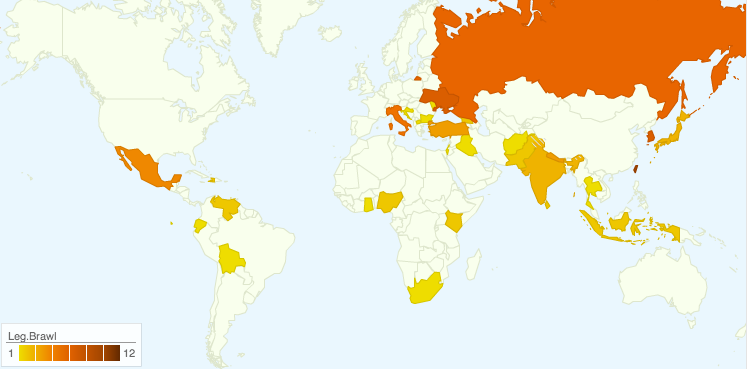
\includegraphics[width = 13cm]{incidence_map.png}
\end{figure}

%%%%%%%%%%%%%% Describing violence in National Legislatures
\section{Describing Violence in National Legislatures Around the World}

To systematically study legislative violence at a global scale I used the Google News Archive\endnote{See {\url{http://news.google.com/archivesearch}}.} to create a data set of {\emph{physical fights between legislators in national legislative chambers}}.\endnote{The Google News Archive search was conducted in Spring 2011. Please contact me for a complete list of sources and search terms.} This resulted in a data set of 88 incidences of legislative violence in 30 countries between 1981 and Winter 2011. We can see in Figure \ref{leg_map} that these events have occurred in many countries around the world. They do not appear to be confined to any one cultural group or region as a cultural explanation would predict. 

Violence is nonetheless not evenly distributed across countries. I observed 30 countries having incidences of legislative violence, but over 60 percent of these fights occurred in eight countries with four or more total legislative brawls. Before moving on to the regression analysis it is useful to first examine the simple associations between proportional outcomes and democratic age. In Figure \ref{framework_empirical} I plot two variables measuring these concepts with the entire sample of countries--in the following parametric analysis we will only look at elected legislatures. Each point represents a country-year. 

The association between age of democracy and violence is clear in Figure \ref{framework_empirical}. Its notable that all of the observed incidences of violence took place in legislatures with disproportional seat distributions.\endnote{Disproportionality is measured with the Gallagher disproportionality score \citep[][see the discussion below for further details]{Gallagher1991,Gallagher2012}.}. Similarly, older democracies (approximately 55 years or more old)\endnote{Democratic age is determined by how many years a country had Polity scores greater than 5. Five is the qualitative point the creators of the Polity data set choose for determining if a country is democratic or not \citep{Marshall2009}.} were never observed having legislative brawls.\endnote{This is not to say that physical fights between legislators never happen in these countries. For example, during the writing of this paper a member of the United Kingdom Parliament assaulted a number of people at Palace of Westminster pub. See {\url{http://www.guardian.co.uk/politics/2012/mar/12/eric-joyce-labour-membership}}.}

While it appears that having disproportional electoral outcomes or a new democracy is not necessary for legislative violence, based on the data, it looks as though having \emph{both} of them is necessary for violence. For example, South Korea is an example of a country with such a ‘perfect storm’. It has both a new democracy and a fairly disproportional electoral outcomes.\endnote{South Korea’s average disproportionality as measured by the Gallagher Index from 2000 until 2011 was 12.7. This places it in the upper 25 percent of observations with democratic legislatures.} It became a democracy within the past 20 years. Conversely, countries that have \emph{either} proportional outcomes \emph{or} democracy can compensate for an absence of the of another. For example the United Kingdom has a fairly disproportionate electoral system,\endnote{It had an average Gallagher disproportionality of 16.5 from 2000 to 2011.} but no violence. One reason for this might be that it has a very old democracy both left-leaning Labour and right-leaning Conservative parties have had experience in government and can expect to be in government in the future. They can therefore more easily view parliamentary procedures as fair and legitimate. Conversely, no incidences of violence were observed in South Africa's new democracy. However, they have very proportional electoral outcomes.\endnote{South Africa’s average disproportionality was 0.29 from 2000 until 2011, one of the lowest observed in the sample.} So it may be easier for opposition legislators to view parliamentary rules and decisions as fair and legitimate.

This brief tour of descriptive statistics and  suggests that violence between legislators does not occur randomly. Instead violence does appears to be a characteristic of countries with disproportional electoral outcomes and new democracies.

%%%%%%%%%%%%%%%% Scatterplot of Disproportionality, AgeDem, and Violence %%%%%%%%%%%%%%%%%%%%%%%%
\begin{figure}[t]
    \caption{Scatterplots of Disproportionality, Government Majority, Age of Democracy, and Violence in the Full Sample.}  
    \label{framework_empirical}
    \begin{center}

\begin{knitrout}
\definecolor{shadecolor}{rgb}{0.969, 0.969, 0.969}\color{fgcolor}
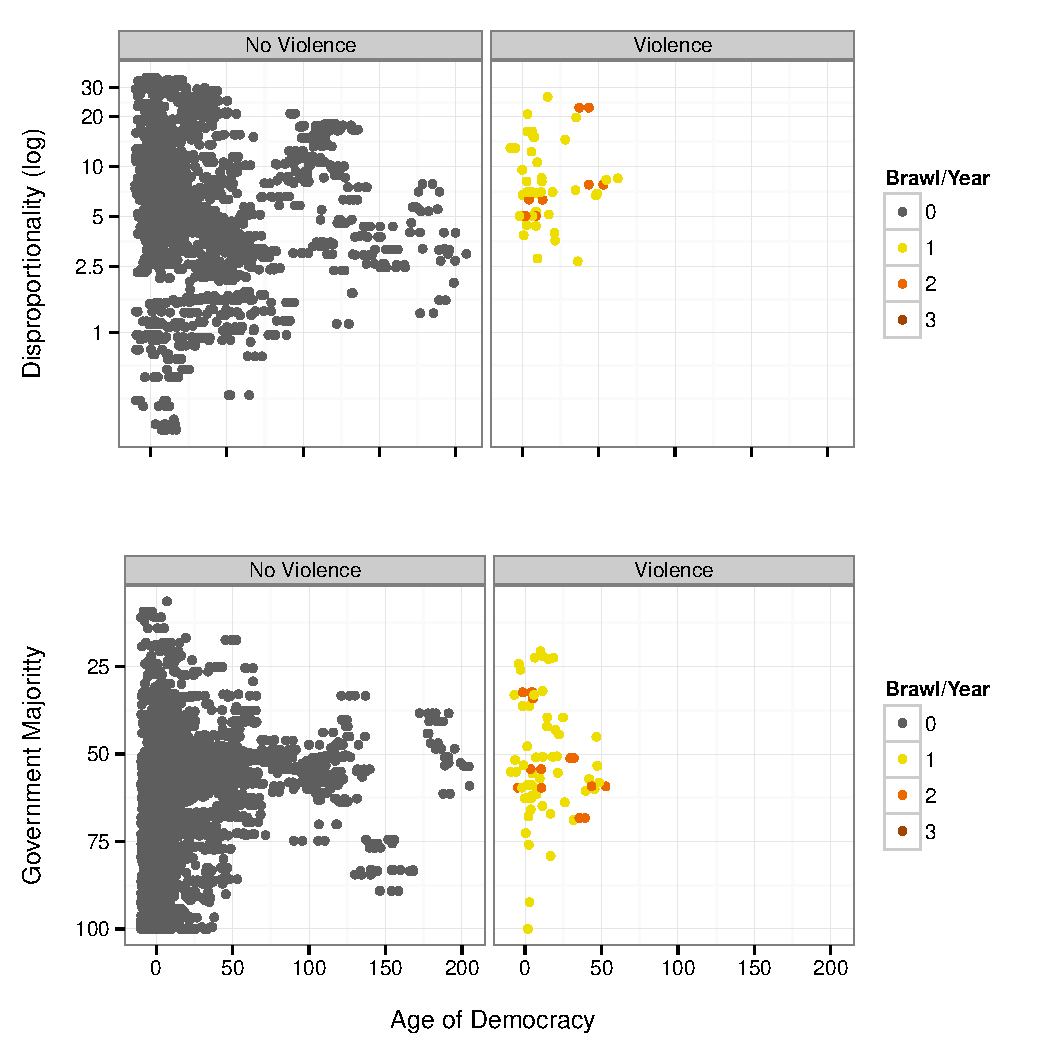
\includegraphics[width=0.8\linewidth]{figure/FrameworkEmpirical} 

\end{knitrout}

    \end{center}
    \begin{singlespace}
        {\scriptsize{Each point represents a country-year. \\ The data is from a sample of 200 countries between 1981 and 2009. The points are jittered horizontally.}}
    \end{singlespace}

\end{figure}

%%%%%%%%%%%%%%%%%%%%%%%%%%%%%%%%%%%%%%%%%%%%%%%%%%%%%%%%%%%%%%%%%%%%%%%%%%% Empirical Analysis
\section{Empirical Analysis: What is Associated with Legislative Brawls?}

To be able to more closely and robustly examine on a global scale I use incidences of legislative brawls as the dependent variable in a series of rare events logistic regression models \citep{KingRareEvents2001, KingRareEventsPA2001}. Following Gary King's \citeyearpar{King1995} recommendation, full replication data and code used for all of the analyses can be found in this paper's source code files.\endnote{Full replication files can be found at \url{https://github.com/christophergandrud/LegislativeViolence}.}

%%%%%%%%%%%%%%%%%%%%%%%%%%%%%%%%%%%%%%%%%%%% Independent variables
\subsection{Right-hand Variables}

I included a number of political, societal, and economic variables in the regression models to test if the associations we saw earlier are actually spurious and other factors, such as a lack of societal trust or legislative immunity are associated with legislative violence. Variable descriptions and sources are summarized in Table \ref{var_summary} in the Appendix. In the interest of transparency, the table includes all of the variables that I have included in all versions of the models, even those not shown.\endnote{Estimates from a number of them are not shown for simplicity. In general, these variables did not generate statistically significant results and it was theoretically unclear how they would influence legislative violence.} A matrix illustrating the variables' correlations can be found in Figure \ref{corrmatrix} in the Appendix. This figure also includes the variables' observed minimum and maximum values for reference. 

We already saw possible associations between the age of democracy and incidences of violence. As mentioned earlier, I measure the {\emph{age of a democratic regime}} as the number of years a country's Polity score is greater than five.

Older democracies are more likely to have higher proportions of legislators who have actually experienced being both winners and losers. I would have liked to more directly model the effects of legislator tenure by including some measures of the time legislators are in office. Unfortunately, I was unable to find data on legislator tenure for the range of countries included in the sample. As a proxy I include the {\emph{tenure of the shortest serving veto player}} variable from the Database of Political Institutions (DPI) \citep[updated to 2010]{DPI2001}. In this data set veto players are either the prime minister and major parliamentary parties or the president and the largest legislative party.

I use two variables to examine the relationship between the fairness of electoral outcomes and violence. The first is purely institutional: a simple dummy of whether or not a country's legislature is elected by some form of {\emph{proportional electoral system}}. The variable is from the DPI database. As noted earlier, simply looking at the electoral mechanics confuses mechanisms with outcomes. So, more importantly, I use the standard Least Squares or Gallagher Index \citep[see][]{Gallagher1991} to measure realized {\emph{electoral disproportionality}}.\endnote{Carey and Hix refer to the Index as the ``established means of measuring proportionality in electoral systems" \citeyearpar[387]{Carey2011}. The index is calculated for each election with the following equation: $ \mathrm{LS} = \sqrt{\frac{1}{2}\displaystyle\sum_{i=1}^{n} (v_{i}-S_{i})^2}$, where $V_i$ is the vote share for party $i$ and $S_{i}$ is party $i$'s seat share.} To gain maximum coverage, I compiled the data from both \cite{Gallagher2012} and \cite{Carey2011}.\endnote{Full details can be found at {\url{http://christophergandrud.github.com/Disproportionality_Data/}}.} A country's disproportionality score is treated as constant from the year of an election until the year before the following election. Higher values on the Gallagher Index indicate more disproportional, i.e. less fair electoral outcomes. 

As we saw in Figure \ref{framework_empirical} there appears to be a very strong negative correlation between very low levels of disproportionality and legislative violence. No instances of violence were observed in countries with a disproportionality score of less than about 2.5.\endnote{Though the observed range of disproportionality scores goes from almost 0 to 30, countries with scores less than 2.5 are not outliers. About 42 percent of county-years in the sample had scores of 2.5 or smaller.} This is similar to Marien's \citeyearpar{Marien2011} finding regarding disportionality and political trust discussed above. To capture a possible disproportionality threshold effect--where very low disproportionality is associated with stronger feelings of fairness and legitimacy--I created a higher and lower disproportionality dummy variable. County-years with disproportinality greater than or equal to the observed median (6) are coded as having higher disproportionality and those with scores lower than 6 are coded as having very low disproportionality.\endnote{Models were estimated with the continuous disproportionality measure. The parameter estimates were not statistically significant.} 

\paragraph{Other Variables}

To get a sense of the size of the governing majority I include the government {\emph{majority}} variable (from DPI) that simply measures the seats held by governing parties as a proportion of all seats. I transformed the variable from a proportion to a percentage to ease interpretation. 

I also investigated the possibility that a number of political, institutional, and cultural variables may actually be associated with legislative violence and that the key framework variables discussed so far actually have spurious associations. 

Legislators may be less likely to attack one another if they know that they could be arrested for assault. To examine this possibility I include Fish and Koening's \citeyearpar{Fish2009} dichotomous \emph{legislator immunity} variable. It equals one if national legislators are immune from arrest and/or prosecution and zero otherwise. Unfortunately, their data only captures legislative immunity in 2007. I extrapolated the 2007 value of the variable to the other observation years.\endnote{I also considered using the legislator immunity variable from the Comparative Constitutions Project \citep{ElkinsCCP2010}. However, the coding of the immunity variable is vaguer than Fish and Koening's and only deals with constitutionally mandated immunity.} We should therefore approach results from this variable with some caution since it might not be a valid indicator for all country-year observations.

To examine the relationships between societal-level values and legislative violence I rely primarily on data from the World Values Survey \citep{WVS2009}. Over the course of his research, Ingelhart has found that his composite {\emph{self-expression}} indicator was the best way to capture cultural and normative differences between democracies and non-democracies. Societies have high self-expression scores if they emphasize ``liberty and participation, public self-expression, tolerance of diversity, interpersonal trust, and life satisfaction" \citep[64]{Inglehart2003}. I focus on both the self-expression variable and the component {\emph{trust}} variable\endnote{Higher values on the trust variable indicate less trust.} from World Values Survey because it makes the most intuitive sense that legislators from societies that are very trusting may be less likely to resort to violence in the legislative chamber. Following \cite{Inglehart2003} I average the variables across individual participants within countries and survey waves. I only use the third through fifth survey waves\endnote{The surveys were taken in the following years: \\ Wave 3: 1994--1998 \\ Wave 4: 1999--2004 \\ Wave 5: 2005--2007} as the first two waves have very poor coverage. I used wave 3 for all years before 1998, wave 4 for all years between 1999 and 2004 and wave 5 onward. 

To assess any effect of coalition compared to single-party governments I included the DPI {\emph{government fractionalization}} variable. It is the probability that two randomly picked deputies in the government are from different parties. I used the fractionalization variable to create an indicator of {\emph{single-party}} government. It is simply a dummy equaling one if fractionalization was zero, i.e. all governing legislators were from the same party. In general single party governments probably are better able to pass policies very close to their ideal preferences. This could heighten losers' losses. However, all single party governments are not created equal. Some parties may act as umbrella parties that incorporate many different factions. While others are narrowly focused on a particular constituency. 

In early models I also included standard measures of the \emph{effective number of parliamentary parties} by votes and by seats \citep[see][]{Laakso1979, Taagepera1989}. The data was taken from \cite{Carey2011}\endnote{Their data is mostly from \cite{Golder2005}. Please see their notes for further details.} before 2004 and from \cite{Gallagher2012} afterwards. Both of these measures indicate how fragmented a parliamentary party system is. Higher scores indicate that there are more parties that win either votes or seats.

To examine whether or not national legislative losers may be dissuaded from legislative violence because there is a possibility of gaining power at a provincial-level, I include the \emph{federalism} dummy variable from \cite{Carey2011}.\endnote{Their data is mostly from \cite{Adsera2003}. Please see their notes for further details.} I updated this from 2004 until the end of the observation period.

In many cases there are considerable interactions between these factors, parliamentary rules and the distribution of interests across a country that could influence violence. For example, presidential systems that give relatively equal power to both the president and legislature could be much more consensual than a single party majority parliamentary system if the president and legislature are controlled by different parties. I attempted to capture these sorts of interactions in the analysis, but this is empirically difficult. Given the small number of actual observed incidences of legislative violence there simply might not be enough information in the data to draw meaningful conclusions about these types of relationship \citep[see][]{Brambor2006}.

I include a number of other societal-level variables to help further defend against omitted variable bias. Conflict in more ethnically or economically divided societies may be generally more intense. These conflicts may spill over into legislatures where they precipitate violence between members. I include Alesina et al.'s \citeyearpar{Alesina2003} {\emph{ethnic fractionalization}} data to account for the fact that a legislature's composition in terms of its fractionalization is not only a function of political institutions, but also social divisions \citep{Neto1997, Mozaffar2003}. The variable measures the probability that two randomly selected members of society will be from different ethnic groups. Higher values indicate more societal fractionalization. To capture similar possible effects of economic divisions, I include {\emph{Gini coefficients of economic inequality}} from \cite{UNU2008}.\endnote{Note, for country-years with missing data I assumed that the Gini Coefficient remained constant from the last year there is data for the country, unless the span was ten years or more. If this was the case they were treated as missing.} Finally, as is common in cross-country analyses, I also include {\emph{gross domestic product per capita}} in some of the models. This data is from the World Bank's International Development Indicators \citeyearpar{WorldBank2011} and is in thousands of United States dollars.

%%%%%%%%%%%%%%%%%%%%%%%%%%%%%%%%%%%%%%%%%%%% Empirical Model
\subsection{Parametric Model: Rare Logistic Regression}

Legislative brawls are rare. The overwhelming majority of legislatures, most of the time do not break out into physical fights. The rarity of legislative brawls creates some empirical problems. Standard logistic regression techniques can ``sharply underestimate the probability of rare events" \cite[137]{KingRareEventsPA2001}. \cite{KingRareEventsPA2001} demonstrate that in logit analysis with relatively very fewer observed events than nonevents--many more 0s than 1s--estimated regression coefficients will be too small. Furthermore, standard methods for computing event probabilities with logistic regression produce results biased in the same direction as the coefficient estimates. To overcome this problem they propose a bias-corrected logistic model for rare events data--rare logistic regression. I use this method below.\endnote{If there is no rare event bias, rare events logistic regression will produce results similar to a standard logit analysis. Please see King and Zeng \citep[147--148]{KingRareEventsPA2001} for a more detailed discussion of $\mathrm{Bias}(\hat\beta)$.}

%%%%%%%%%%%%%%%%%%%%%%%%%%%%%%%%%%%%%%%%%%%% Analyses


\subsection{Results}

What is associated with legislative violence? To estimate the rare events bias corrected logit regressions for this paper I used the {\tt{relogit}} model from the {\tt{R}} package Zelig \citep{IMAIKingZelig2008} with data that was in country-year format.\footnote{Country-years with more than one act of violence are given multiple records. See below for a discussion of how the standard errors were adjusted to address statistical issues related to this.} Furthermore, to get a better understanding of the magnitude of the estimated relationships between the right-hand variables and violence, I also used Zelig to predict incident probabilities with 1000 simulations per fitted value \citep[see][]{King2002}. Predicted probabilities for various fitted values of the main variables of interest with robust results are shown in Figure \ref{pred_prob}. These give us a substantively meaningful sense of estimated effects' magnitudes. Selected regression coefficient point estimates and standard errors can be found in Table \ref{outputTable.dem}. Because the variables are recorded as country-years, all of the results should be interpreted in terms of the predicted effect of a variable on the probability of legislative violence in a given year.

I constricted the sample to include only country-years with elected legislatures. Data on whether or not a legislature was elected is from the DPI {\emph{Legislative Indices of Electoral Competitiveness}} variable. Using this criteria constricted the number of legislative violence incidences from 88 to 72 largely because DPI does not have data for 2010 and 2011.\endnote{I used the existing proportion of all observations with legislative violence in the time constricted sample 1.7 percent of observations up until 2010 had violence ($\tau = \frac{72}{4152} = 0.017$). for prior correction in the rare events logistic regressions \citep[see][]{KingRareEventsPA2001}.}

I observed relatively few incidences of violence in the 1980s.\endnote{There were only 8 observed incidence before 1990.} This is probably because news articles from before the 1990s have not been made available on the internet with the same frequency as those written from the 1990s. To examine any estimation biases this sampling bias might create I ran the regressions on a further constricted sample of elected legislatures. The sample included country-years with elected legislatures from 1990.\endnote{For prior correction I used the observed number of violent incidences from 1990. There were 64 observed incidences of violence and 2778 country-years from 1990 through 2009 in the sample, so: $\tau = \frac{64}{2778} = 0.023$.} The results were broadly similar across the different samples. 

Individual observations are clearly correlated within countries and years, especially when there were multiple acts of violence in a country in a year. To address this issue I used robust standard errors \citep{Golder2006, Mainwaring2007}. Standard errors were adjusted using \cite{Lumley1999} weighted empirical adaptive variance estimators (WEAVE) where the true dependence structure does not need to be specified prior to running the analysis.\endnote{Also, using WEAVE to find robust standard errors allowed me to take advantage of Zelig's ability to simulate quantities of interest. Results were very similar to those from estimating the same models in Stata using {\tt{relogit}} with the {\tt{cluster(country)}} option. Please contact me for tables comparing the two sets of results.} 

%%%%%%%%%%%%%%%% Run Analyses %%%%%%%%%%%%%%%%%%%%%%%%


%%%%%%%% Elected Legislatures Results Table
\begin{table}
\caption{Legislative Violence Rare Events Logistic Regression Results (Elected Legislature from 1980)}
\label{outputTable.dem}
\begin{center}

\begin{tabular}{l c c c c c c c }
\hline
                         & A1 & A2 & A3 & A4 & A5 & A6 & A7 \\
\hline
(Intercept)              & $-3.25^{***}$ & $-1.37$       & $-0.54$       & $-4.03^{***}$ & $10.52^{**}$  & $5.05$             & $4.71$            \\
                         & $(0.20)$      & $(0.80)$      & $(6.42)$      & $(1.04)$      & $(3.75)$      & $(2.85)$           & $(2.85)$          \\
High Proportionality     & $-0.92^{**}$  & $-1.42^{***}$ & $-2.40^{***}$ & $-1.05^{**}$  & $-2.06^{**}$  &                    &                   \\
                         & $(0.34)$      & $(0.37)$      & $(0.71)$      & $(0.38)$      & $(0.63)$      &                    &                   \\
Dem. Age                 & $-0.02^{*}$   & $-0.02^{*}$   & $-0.04^{**}$  & $-0.02^{*}$   & $-0.03^{**}$  & $-0.02$            & $-0.02$           \\
                         & $(0.01)$      & $(0.01)$      & $(0.01)$      & $(0.01)$      & $(0.01)$      & $(0.01)$           & $(0.01)$          \\
Majority Size            &               & $-0.04^{***}$ & $-0.01$       &               & $0.00$        & $0.01$             & $0.01$            \\
                         &               & $(0.01)$      & $(0.02)$      &               & $(0.01)$      & $(0.01)$           & $(0.01)$          \\
Leg. Immunity            &               & $-0.54$       &               &               &               &                    &                   \\
                         &               & $(0.34)$      &               &               &               &                    &                   \\
Shortest VP Tenure       &               & $-0.08$       &               &               &               &                    &                   \\
                         &               & $(0.08)$      &               &               &               &                    &                   \\
PR Electoral System      &               & $1.07^{*}$    &               &               &               &                    &                   \\
                         &               & $(0.51)$      &               &               &               &                    &                   \\
Self Expression          &               &               & $8.32$        &               &               &                    &                   \\
                         &               &               & $(4.79)$      &               &               &                    &                   \\
Trust                    &               &               & $-7.29^{**}$  &               & $-8.65^{***}$ & $-5.61^{**}$       & $-5.47^{**}$      \\
                         &               &               & $(2.26)$      &               & $(2.27)$      & $(1.75)$           & $(1.75)$          \\
Ethnic Frac.             &               &               & $2.18$        &               &               &                    &                   \\
                         &               &               & $(1.23)$      &               &               &                    &                   \\
No. of Parties           &               &               &               & $0.15$        &               &                    &                   \\
                         &               &               &               & $(0.10)$      &               &                    &                   \\
Parliamentary            &               &               &               & $0.38$        &               &                    &                   \\
                         &               &               &               & $(1.06)$      &               &                    &                   \\
Presidential             &               &               &               & $0.49$        &               &                    &                   \\
                         &               &               &               & $(1.04)$      &               &                    &                   \\
Federal                  &               &               &               & $0.81$        &               &                    &                   \\
                         &               &               &               & $(0.42)$      &               &                    &                   \\
Gov. Frac.               &               &               &               & $-0.21$       &               &                    &                   \\
                         &               &               &               & $(0.73)$      &               &                    &                   \\
GINI                     &               &               &               &               & $0.05$        & $0.04$             & $0.04$            \\
                         &               &               &               &               & $(0.03)$      & $(0.02)$           & $(0.02)$          \\
GDP per Capita           &               &               &               &               & $-0.02$       & $-0.03$            & $-0.03$           \\
                         &               &               &               &               & $(0.03)$      & $(0.03)$           & $(0.03)$          \\
Very High Prop.          &               &               &               &               &               & $1049336.00^{***}$ & $910918.23^{***}$ \\
                         &               &               &               &               &               & $(870.67)$         & $(1554.72)$       \\
Dem. Age*Very High Prop. &               &               &               &               &               &                    & $21107.61^{***}$  \\
                         &               &               &               &               &               &                    & $(19.39)$         \\
\hline
AIC                      & 413.50        & 386.32        & 185.32        & 354.70        & 201.82        & 212.31             & 214.31            \\
BIC                      & 430.05        & 424.75        & 216.90        & 397.68        & 234.27        & 244.75             & 251.39            \\
Log Likelihood           & -203.75       & -186.16       & -85.66        & -169.35       & -93.91        & -99.15             & -99.15            \\
\hline
\multicolumn{8}{l}{\scriptsize{\textsuperscript{***}$p<0.001$, 
  \textsuperscript{**}$p<0.01$, 
  \textsuperscript{*}$p<0.05$}}
\end{tabular}


\end{center}
{\scriptsize{
    Standard errors in parentheses. All models use robust (WEAVE) standard errors. \\
    Assembly-Elected Presidential system is the reference category for government system variables (Presidential and Parliamentary). \\
}}
\end{table}

%%%%%%%% Elected Legislatures Results Table from 1990
\begin{table}
\caption{Legislative Violence Rare Events Logistic Regression Results (Elected Legislature from 1990)}
\label{outputTable.1990}
\begin{center}

\begin{tabular}{l c c c c c c c }
\hline
                         & B1 & B2 & B3 & B4 & B5 & B6 & B7 \\
\hline
(Intercept)              & $-3.24^{***}$ & $-1.12$      & $-2.33$      & $-4.01^{***}$ & $10.52^{*}$   & $5.91$             & $5.47$            \\
                         & $(0.22)$      & $(0.85)$     & $(6.45)$     & $(1.05)$      & $(4.16)$      & $(3.30)$           & $(3.29)$          \\
High Proportionality     & $-0.78^{*}$   & $-1.18^{**}$ & $-2.02^{**}$ & $-0.98^{*}$   & $-1.64^{**}$  &                    &                   \\
                         & $(0.36)$      & $(0.39)$     & $(0.71)$     & $(0.40)$      & $(0.63)$      &                    &                   \\
Dem. Age                 & $-0.02^{*}$   & $-0.02^{*}$  & $-0.04^{*}$  & $-0.02^{*}$   & $-0.03^{*}$   & $-0.03$            & $-0.03$           \\
                         & $(0.01)$      & $(0.01)$     & $(0.02)$     & $(0.01)$      & $(0.02)$      & $(0.02)$           & $(0.02)$          \\
Majority Size            &               & $-0.04^{**}$ & $-0.02$      &               & $-0.01$       & $0.00$             & $0.00$            \\
                         &               & $(0.01)$     & $(0.02)$     &               & $(0.02)$      & $(0.01)$           & $(0.01)$          \\
Leg. Immunity            &               & $-0.36$      &              &               &               &                    &                   \\
                         &               & $(0.37)$     &              &               &               &                    &                   \\
Shortest VP Tenure       &               & $-0.07$      &              &               &               &                    &                   \\
                         &               & $(0.08)$     &              &               &               &                    &                   \\
PR Electoral System      &               & $0.68$       &              &               &               &                    &                   \\
                         &               & $(0.53)$     &              &               &               &                    &                   \\
Self Expression          &               &              & $9.15$       &               &               &                    &                   \\
                         &               &              & $(4.80)$     &               &               &                    &                   \\
Trust                    &               &              & $-6.48^{**}$ &               & $-8.58^{***}$ & $-6.17^{**}$       & $-5.99^{**}$      \\
                         &               &              & $(2.48)$     &               & $(2.52)$      & $(2.03)$           & $(2.02)$          \\
Ethnic Frac.             &               &              & $1.65$       &               &               &                    &                   \\
                         &               &              & $(1.33)$     &               &               &                    &                   \\
No. of Parties           &               &              &              & $0.15$        &               &                    &                   \\
                         &               &              &              & $(0.10)$      &               &                    &                   \\
Parliamentary            &               &              &              & $0.20$        &               &                    &                   \\
                         &               &              &              & $(1.08)$      &               &                    &                   \\
Presidential             &               &              &              & $0.60$        &               &                    &                   \\
                         &               &              &              & $(1.04)$      &               &                    &                   \\
Federal                  &               &              &              & $0.53$        &               &                    &                   \\
                         &               &              &              & $(0.49)$      &               &                    &                   \\
Gov. Frac.               &               &              &              & $-0.08$       &               &                    &                   \\
                         &               &              &              & $(0.77)$      &               &                    &                   \\
GINI                     &               &              &              &               & $0.06^{*}$    & $0.05$             & $0.05$            \\
                         &               &              &              &               & $(0.03)$      & $(0.03)$           & $(0.03)$          \\
GDP per Capita           &               &              &              &               & $-0.01$       & $0.00$             & $-0.01$           \\
                         &               &              &              &               & $(0.03)$      & $(0.04)$           & $(0.04)$          \\
Very High Prop.          &               &              &              &               &               & $1388319.80^{***}$ & $946603.56^{***}$ \\
                         &               &              &              &               &               & $(998.49)$         & $(1929.62)$       \\
Dem. Age*Very High Prop. &               &              &              &               &               &                    & $30047.00^{***}$  \\
                         &               &              &              &               &               &                    & $(23.23)$         \\
\hline
AIC                      & 343.07        & 322.39       & 153.00       & 288.84        & 162.37        & 168.20             & 170.20            \\
BIC                      & 358.82        & 358.92       & 182.71       & 329.60        & 192.83        & 198.66             & 205.01            \\
Log Likelihood           & -168.54       & -154.20      & -69.50       & -136.42       & -74.19        & -77.10             & -77.10            \\
\hline
\multicolumn{8}{l}{\scriptsize{\textsuperscript{***}$p<0.001$, 
  \textsuperscript{**}$p<0.01$, 
  \textsuperscript{*}$p<0.05$}}
\end{tabular}


\end{center}
{\scriptsize{
    Standard errors in parentheses. All models use robust (WEAVE) standard errors. \\
    Assembly-Elected Presidential system is the reference category for government system variables (Presidential and Parliamentary). \\
}}
\end{table}

I avoid focusing on models that include highly correlated variables \citep[see][]{Achen2002, Schrodt2006}. In these models (not shown), as the statistical literature predicts, the coefficient estimates and standard errors change dramatically for many of the variables, because they are highly correlated. Models with interaction terms are not shown because they generally did not produce meaningful results. This may be because there are genuinely no conditional relationships between the variables of interest or there is not enough information in the data to reveal these relationships given the small number observed incidences of violence. Because of this ambiguity I avoid directly presenting and attempting to interpret interaction estimates. 

%%%%%%%%%%%%%%%% Predicted Probability Graphs %%%%%%%%%%%%%%%%%%%%%%%%
\begin{figure}[t]
    \caption{Predicted Probability of Legislative Violence in Elected Legislatures}  
    \label{pred_prob}
    \begin{center}

    %\includegraphics[width = \textwidth]{leg_violence_paper-PredProb}

\begin{knitrout}
\definecolor{shadecolor}{rgb}{0.969, 0.969, 0.969}\color{fgcolor}
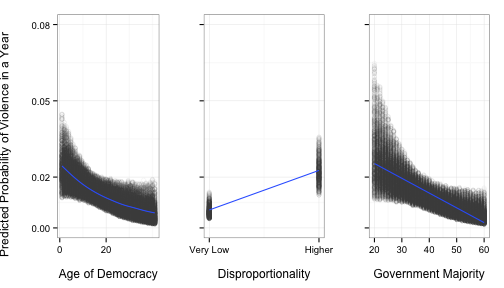
\includegraphics[width=0.8\linewidth]{figure/predProb} 

\end{knitrout}

    \end{center}
    \begin{singlespace}
      {\scriptsize{The graphs show the middle 95\% of 1000 simulations at each fitted value of the variables. The simulations use Model B2 with the sample constricted to observations from 1990. See Table \ref{outputTable.1990}.}}
    \end{singlespace}
\end{figure}

\paragraph{Age of Democracy}
Corroborating what we saw in Figure \ref{framework_empirical}, the rare events logit analyses generally indicate that older democracies tend to have less legislative violence. The statistical significance of the democratic age variable is weak in a model by itself, but improves when institutional variables are included. In all models the direction of the relationship is negative: the older the democracy, the less likely violence is to occur. This is what we expect from the framework presented earlier. More interesting than simple statistical significance or coefficient point estimates is the magnitude of and uncertainty surrounding the democratic age/violence relationship. To get a sense of this estimated relationship and the uncertainty around it \citep[see][]{King2000} I plotted the predicted probabilities of having a legislative brawl in Figure \ref{pred_prob} using information from Model 15 with the sample constricted to observations from 1990.\endnote{To estimate these probabilities I ran 1000 simulations for each value of the democratic age variable between age 0 and 85. Other covariates were held at their means.} Very young democracies are predicted to have about a two percent probability of experiencing legislative violence in a given year. The probability of violence decreases steadily from there. The predicted probability of violence becomes largely indistinguishable from zero--i.e. no probability of violence--shortly after a democracy turns 50 years old.

Looking at the tenure of the newest veto player, we find some evidence that countries with longer serving veto players are less likely to have violence. This finding fits somewhat with the idea that as actors have more experience being both winners and losers they become less likely to use extra-procedural means, such as violence. Note that the finding is not robust in fuller models.

\paragraph{Disproportionality}
Results from models using the dummy {\emph{high proportionality}} variable indicate that highly proportional electoral outcomes are associated with less legislative violence. This finding is robust\endnote{i.e. it is statistically significant at least at the 5\% significance level.} in all model specifications. This confirms what we saw in Figure \ref{framework_empirical}. Violence is very rare in countries with Gallagher scores below the median--6--and there is a something of a cutoff point--around 2.5--below which these highly proportional countries were not observed to have had any violence. The middle plot in Figure \ref{pred_prob} shows the simulated probability of having legislative violence when disproportionality is high or very low. The predicted probability of having violence when disproportionality is greater than or equal to 6 is a little over two percent in a given year. This probability is similar to that of very young democracies. Countries with disproportionality less than 6 had almost no probability of violence over a year.

\paragraph{Governing Majorities}
I also found a negative relationship between the size of governments' legislative majorities and violence. Perhaps this finding is being driven by more legislatures with hegemonic and very powerful parties that control virtually all of the seats. To rule this possibility out, I reran the models where observations with government majorities greater than 90 percent were dropped and controlled for level of democracy. The results (not shown) nonetheless persisted.\endnote{Please contact the author for these results tables.} We can see in Figure \ref{pred_prob} that the predicted probability of violence in legislatures with small minority governments is relatively high, similar to that of young democracies and highly disproportional legislatures. Losers in legislatures where the government controls well under 50 percent of the seats would likely view the minorities control of the agenda as being unfair and illegitimate--even if the minority government has a constrained ability to affect policy change. This might prompt them to use violence in an attempt to block the minority governments control of the agenda. 

It's important to note that the government majority variable was not significant in the models that also included societal-level trust. Substantively, it's unclear why this might be, though it does bring the robustness of the relationship between government majority size and legislative violence into question. 

\paragraph{Cultural and Societal Variables}

As just mentioned the measure of societal-level trust was robust and significant in all of the models in which it was included. The negative direction of the relationship is what we would expect. More trusting societies, have legislatures with less violence. This finding generally fits within this paper's broader framework in that legislators that are more trusting might be more inclined to believe that other legislative actors will not unfairly use legislative procedures. Nonetheless, it takes a bit of a leap to believe that the mean level of trust found using a national-level survey accurately reflect the values held by elite individuals in legislatures. Further work is needed to make stronger conclusions about the relationships between trust and the propensity for legislative violence. This research could possibly use individual legislator surveys that would allow us to directly measure the distribution of values among actual legislators. In general the other cultural and other societal-level variables, such as wealth and ethnic fractionalization were not found to be robustly associated. 

\paragraph{Other Political and Institutional Variables}
Results for other political and institutional variables were largely not statistically significant. Legislative immunity from arrest and/or prosecution is not significantly associated with legislative violence. We should approach this result cautiously since the Fish and Koening immunity variable is based on observations in 2007 and therefore might not be a valid indicator for many country-years.

Neither presidential nor parliamentary systems are more associated with violence.\endnote{The coefficient estimates are statistically significant in the garbage can model, but this result is likely an artifact of the system variable being highly correlated with other variables. The estimate for mixed systems in particular changes dramatically and is largely nonsensical.} This seems to corroborate Horowitz's \citeyearpar{Horowitz1990} argument that the association between executive regime and distribution of power is not clear cut. The observed positive relationship between proportional electoral systems was relatively weak and virtually non-existent when disproportionality was included. This fits with the argument that we should focus on electoral outcomes rather than simple mechanics. Neither effective number of parties variables, the basic continuous government fractionalization variable nor the more substantively interesting single-party government variables are `statistically significant' in the analyses. Likewise, federalism did not appear to be related to legislative violence. All of these variables are not as directly related to fairness at a theoretical level, compared to disproportionality and, to a lesser extent, governing majorities. So it should not come as too much of a surprise to find that they are more loosely, if not at all, associated with legislative violence.

%%%%%%%%%%%%%%%%%%%%%%%%%%%%%%%%%%%%%%%%%%%% Conclusions
\section*{Conclusions: What Keeps Legislators Two Sword Lengths Apart?}

In this paper--the first to systematically examine legislative violence on a global scale--I developed a framework for predicting when legislative violence is more likely. I then empirically tested the framework with a new data set of legislative brawls. In the course of doing this What conclusions can we make from the paper's findings about why legislators are kept `two sword lengths' apart (or not)?

The findings in this paper suggest that countries with highly proportional electoral outcomes rarely experience legislative violence. In the present sample the relationship appears to be subject to a strong threshold effect where countries with Gallagher Index scores below about 5 rarely experience legislative violence and those below 2.5 never did. This corresponds closely to Marien's \cite{Marien2011} finding that political trust is higher in countries with proportional electoral outcomes. 

The proportionality finding is illustrated by the new Southern African democracies, chiefly South Africa and Namibia. Despite having new democratic institutions, very fractious societies, and recent histories of intense armed conflict neither country was recorded to have experienced legislative violence.\footnote{This does not mean that there are no instances of disruption in the South African parliament. However, these have always been nonviolent \cite{Johnson2013}.} When both countries transitioned to democracy they did develop electoral systems that tended to create highly proportional outcomes.\endnote{Namibia's average disproportionality for its years as a democracy is 0.83 and South Africa's is 0.31. South Africa has one of the most proportional systems in the sample.} Perhaps, higher proportionality leads legislators to believe that legislative outcomes are fair enough and extreme extra-procedural measures, like violence, are unwarranted.    

This finding has perhaps the most important potential implications for democratic institutional designers who may want to actively keep legislators two sword lengths apart. Democratic age is partially the result of institutional quality (and perhaps even a lack of legislative violence) and is subject to many factors far outside of the control of democratic planners. Electoral disproportionality is comparatively much more malleable. Proportional electoral systems are the most obvious tool electoral system designers have to increase the correspondence between party's votes and seats \citep{Carey2011}. These systems can be tweaked by increasing district magnitude or altering the formula used to translate votes into seats depending on the distribution of preferences in the electorate. If the findings in this paper are suggestive of an actual relationship between disproportionality and legislative violence then electoral system designers would likely want to aim for a combination of levers that help achieve very proportional outcomes. 

There is still considerable work that can be done to better understand the causes and consequences of legislative violence in democracies. Further case study work can build on the findings here to closely examine the strategic interactions between winners and losers. For example, are their reasons that the legislators may instigate violence or if in government not strongly stop violence it in order to garner media attention? Furthermore, what are the consequences of legislative violence, especially in terms of citizens' perceptions of democratic legitimacy and, indeed, the longterm viability of the democratic regime? These issues should be investigated in future work. 

%%%%%%%%%%%%%%%%%%%%%%%%%%%%%%%%%%%%%%% Appendix

\bibliographystyle{apsr}
\bibliography{LegViolence}

\theendnotes

%%%%%%%%%%%%%%%%%%%%%% Figures Start %%%%%%%%%%%%%%%%%%%%%%%%%%%%%%%%%%%%%%%%%%%%%

\clearpage
\section*{Appendix}


%%%%%%%% Variable source summary table
\begin{table}[!h]
    \begin{center}
    \caption{Variable Summary}
    \label{var_summary}
    \begin{tabular}{l m{7cm} m{3.5cm}}

            \hline
            Variable & Description & Source \\
            \hline \hline
            Disprop & Gallagher Index of Electoral Disproportionality & \cite{Gallagher2012} \& \cite{Carey2011} \\
            ENPS & Effective number of parties by seats & \cite{Gallagher2012} \& \cite{Carey2011} \\
            ENPV & Effective number of parties by votes & \cite{Gallagher2012} \& \cite{Carey2011} \\
            Ethnic Fractionalization & Probability two randomly selected members of society are from the same ethnic group & \cite{Alesina2003} \\
            Federal & Whether a country has a federal system or not & \cite{Carey2011}, updated from 2003 by the author \\           
            GDP/Capita & GDP per capita in thousands of US dollars & \cite{WorldBank2011} \\
            Gov. Fractionalization & Probability that two members of the Government will be from different parties & \cite{DPI2001} \\
            Gini & Gini Coefficient of income inequality & \cite{UNU2008} \\
            Immunity & Whether a legislators are immune from arrest and/or criminal prosecution or not & \cite{Fish2009} \\
            LEIC & Legislative Indices of Electoral Competition. Includes both the existence of a legislature and its electoral competitiveness. & \cite{DPI2001} \\
            Majority & Percentage of legislature controlled by governing parties & \cite{DPI2001} \\
            Polity & Polity IV Score & \cite{Marshall2009} \\
            PR & Whether a country uses a proportional representation electoral system or a plurality system & \cite{DPI2001} \\
            Self Expression & WVS self-expression indicator averaged across country-survey waves & \cite{WVS2009} \\
            System & Government system (parliamentary, presidential, or mixed & \cite{DPI2001} \\
            Tenshort & Tenure of the shortest serving veto player & \cite{DPI2001} \\
            Trust & Average of WVS responses where 1 $=$ most people can be trusted and 2 $=$ you can't be too careful & \cite{WVS2009} \\
            UDS & Posterior Mean Unified Democracy Score & \cite{Pemstein2010} \\
            Violence & Incidences of violence between legislators in the national parliamentary chamber & author \\
            \hline

    \end{tabular}
    \end{center}
    \begin{singlespace}
        Please contact the author for detailed summary statistics.
    \end{singlespace}
\end{table}  

%%%%%%%%%% Correlation matrix %%%%%%%%%% 
\begin{landscape}
\begin{figure}[t]
    \caption{Correlation Matrix for Variables Included in the Analysis (Elected Legislatures)}
    \label{corrmatrix}
    \begin{center}
    
    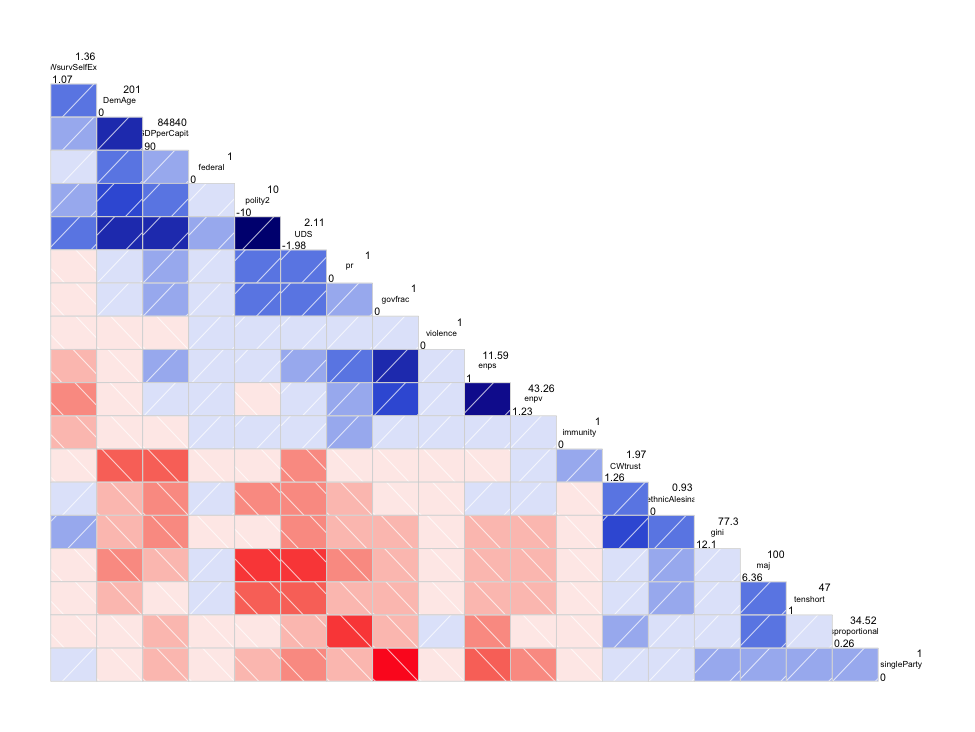
\includegraphics[width = \textwidth]{figure/corScatter.png}  
    %%% corScatter not created every compile to save time %%%
%<<corScatter>>=

%    library(corrgram)  

%    ### Create data set with variables for corrgram
%    vars.corrgram <- c("violence", "system", "DemAge", "maj", "MajCat", "govfrac", "singleParty", "pr", "tenshort", "UDS", "polity2", "ethnicAlesina", "CWtrust", "CWsurvSelfExpr", "disproportionality", "gini", "GDPperCapita", "enps", "enpv", "federal", "immunity")

%    # Subset elected legislature data
%    dem.corrData <- dem[vars.corrgram]

%    # Create corrgram
%    dem.corrgram <- corrgram(dem.corrData, order = TRUE, upper.panel = NULL, diag.panel = panel.minmax)

%@

    \end{center}
    \begin{singlespace}
        {\scriptsize{Redder squares indicate stronger negative bivariate correlations. \\
        Bluer squares indicate stronger positive bivariate correlations. \\
        Numbers in the diagonal squares indicate the minimum and maximum observed values of the variables in the sample.
        }}
    \end{singlespace} 
\end{figure}
\end{landscape}

%%%%%%%%%%%%%%%%%%%%%% Figures End %%%%%%%%%%%%%%%%%%%%%%%%%%%%%%%%%%%%%%%%%%%%%

\end{document}
